\documentclass{article}

% content/resources/templates/preamble.tex
\usepackage[margin=0.6in]{geometry}
\author{Milav Dabgar}
\usepackage{amsmath,amssymb,amsthm}
\usepackage{booktabs}
\usepackage{multirow}
\usepackage{xcolor}
\usepackage{tcolorbox}
\tcbuselibrary{breakable,skins}
\usepackage[colorlinks=true,linkcolor=blue]{hyperref}
\usepackage{titlesec}
\usepackage{enumitem}
\usepackage{tikz}
\usepackage{pgfplots}
\usepackage{circuitikz}
\usepackage[version=4]{mhchem}
\usepackage{longtable}
\usepackage{array}
\usepackage{float}
\usepackage{caption}
\usepackage{listings}

\lstset{
  basicstyle=\small\ttfamily,
  breaklines=true,
  breakatwhitespace=false,
  postbreak=\mbox{\textcolor{red}{$\hookrightarrow$}\space},
  float=false,
  numbers=left,
  numberstyle=\tiny\color{gray},
  numbersep=10pt,
  xleftmargin=2em,
  keywordstyle=\color{blue},
  commentstyle=\color{green!60!black},
  stringstyle=\color{purple},
  backgroundcolor=\color{gray!5},
  showstringspaces=false,
  tabsize=2,
  captionpos=b,
  keepspaces=true,
  columns=flexible
}

\pgfplotsset{compat=1.18}
\usetikzlibrary{shapes,arrows,positioning,calc,patterns,decorations.pathmorphing,decorations.markings,arrows.meta}

% Color scheme
\definecolor{headcolor}{RGB}{0,102,204}
\definecolor{keycolor}{RGB}{220,20,60}
\definecolor{solutioncolor}{RGB}{34,139,34}
\definecolor{mnemoniccolor}{RGB}{148,0,211}
\definecolor{codecolor}{RGB}{0,0,100}

% Spacing
\setlength{\parskip}{3pt}
\setlist[itemize]{nosep}
\setlist[enumerate]{nosep}

% Title formatting
\titleformat{\section}{\Large\bfseries\color{headcolor}}{\thesection}{1em}{}
\titleformat{\subsection}{\large\bfseries\color{headcolor}}{\thesubsection}{1em}{}

% Pandoc tightlist compatibility
\providecommand{\tightlist}{%
  \setlength{\itemsep}{0pt}\setlength{\parskip}{0pt}}

% Pandoc longtable compatibility
\newcounter{none}
\def\thenone{}


% content/resources/templates/english-boxes.tex

% Custom environments
\newtcolorbox{solutionbox}{
 breakable,
 enhanced,
 colback=solutioncolor!5!white,
 colframe=solutioncolor!75!black,
 fonttitle=\bfseries,
 title=Solution
}

\newtcolorbox{solutionboxnobreak}{
 colback=solutioncolor!5!white,
 colframe=solutioncolor!75!black,
 fonttitle=\bfseries,
 title=Solution
}

\newtcolorbox{keyformula}{
 breakable,
 enhanced,
 colback=keycolor!5!white,
 colframe=keycolor!75!black,
 fonttitle=\bfseries,
 title=Key Formula
}

\newtcolorbox{mnemonicboxenv}{
 breakable,
 enhanced,
 colback=mnemoniccolor!5!white,
 colframe=mnemoniccolor!75!black,
 fonttitle=\bfseries,
 title=Mnemonic
}

\newcommand{\mnemonicbox}[1]{%
  \begin{mnemonicboxenv}
    #1
  \end{mnemonicboxenv}
}


% Custom commands for GTU solutions
% This file defines semantic commands for consistent formatting

% Question command with automatic formatting
\newcommand{\question}[2]{%
  \section*{Question #1}%
  \textbf{#2}%
}

% OR question variant
\newcommand{\questionor}[2]{%
  \section*{Question #1 OR}%
  \textbf{#2}%
}

% Proper table environment with caption
\newenvironment{answertable}[1]{%
  \begin{table}[htbp]
  \centering
  \caption{#1}
}{%
  \end{table}
}

% Proper figure environment for diagrams
\newenvironment{answerdiagram}[1]{%
  \begin{figure}[htbp]
  \centering
  \caption{#1}
}{%
  \end{figure}
}

% Semantic markup for key terms
\newcommand{\keyword}[1]{\textbf{#1}}
\newcommand{\code}[1]{\texttt{#1}}
\newcommand{\classname}[1]{\texttt{#1}}
\newcommand{\methodname}[1]{\texttt{#1}}

% Proper quotation marks
\newcommand{\mnemonic}[1]{``#1''}


\title{Data Structure and Application (1333203) - Winter 2023 Solution}
\date{January 18, 2024}

\begin{document}
\maketitle

\questionmarks{1(a)}{3}{Define linked list. List different types of linked list.}

\begin{solutionbox}
\begin{center}
\captionof{table}{Linked List Definition and Types}
\begin{tabulary}{\linewidth}{|L|L|}
\hline
\textbf{Definition} & \textbf{Types of Linked List} \\ \hline
A linked list is a linear data structure where elements are stored in nodes, and each node points to the next node in the sequence & 1. Singly Linked List \\
& 2. Doubly Linked List \\
& 3. Circular Linked List \\
& 4. Circular Doubly Linked List \\ \hline
\end{tabulary}
\end{center}

\begin{center}
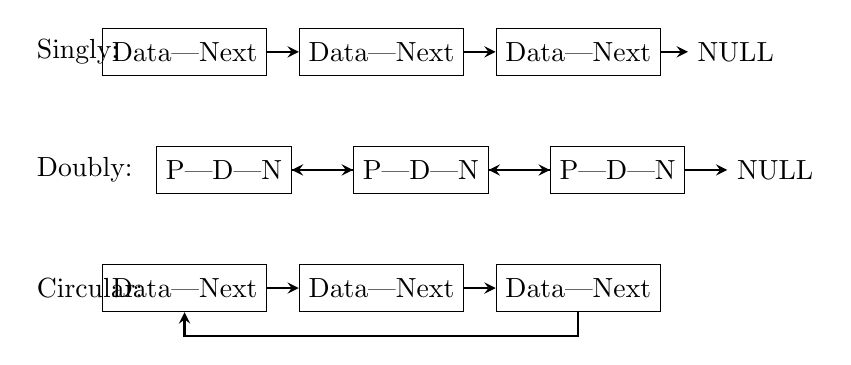
\begin{tikzpicture}[
    listnode/.style={rectangle, draw=black, minimum size=6mm},
    ptr/.style={->, >=stealth, thick}
]
    % Singly
    \node[anchor=west] at (-1, 1.5) {Singly:};
    \node[listnode] (s1) at (1, 1.5) {Data|Next};
    \node[listnode] (s2) at (3.5, 1.5) {Data|Next};
    \node[listnode] (s3) at (6, 1.5) {Data|Next};
    \node (snull) at (8, 1.5) {NULL};
    \draw[ptr] (s1) -- (s2);
    \draw[ptr] (s2) -- (s3);
    \draw[ptr] (s3) -- (snull);

    % Doubly
    \node[anchor=west] at (-1, 0) {Doubly:};
    \node[listnode] (d1) at (1.5, 0) {P|D|N};
    \node[listnode] (d2) at (4, 0) {P|D|N};
    \node[listnode] (d3) at (6.5, 0) {P|D|N};
    \node (dnull) at (8.5, 0) {NULL};
    \draw[ptr] (d1) -- (d2);
    \draw[ptr] (d2) -- (d1);
    \draw[ptr] (d2) -- (d3);
    \draw[ptr] (d3) -- (d2);
    \draw[ptr] (d3) -- (dnull);

    % Circular
    \node[anchor=west] at (-1, -1.5) {Circular:};
    \node[listnode] (c1) at (1, -1.5) {Data|Next};
    \node[listnode] (c2) at (3.5, -1.5) {Data|Next};
    \node[listnode] (c3) at (6, -1.5) {Data|Next};
    \draw[ptr] (c1) -- (c2);
    \draw[ptr] (c2) -- (c3);
    \draw[ptr] (c3.south) -- ++(0,-0.3) -| (c1.south);
\end{tikzpicture}
\captionof{figure}{Types of Linked Lists}
\end{center}
\end{solutionbox}

\begin{mnemonicbox}
\mnemonic{Single, Double, Circle, Double-Circle}
\end{mnemonicbox}

\questionmarks{1(b)}{4}{Explain Linear and Non Linear Data structure in Python with examples.}

\begin{solutionbox}
\begin{center}
\captionof{table}{Linear vs Non-Linear Data Structures}
\begin{tabulary}{\linewidth}{|L|L|L|}
\hline
\textbf{Data Structure} & \textbf{Description} & \textbf{Python Examples} \\ \hline
\textbf{Linear} & Elements arranged in sequential order where each element has exactly one predecessor and successor (except first and last) & Lists: \code{[1, 2, 3]} \newline Tuples: \code{(1, 2, 3)} \newline Strings: \code{"abc"} \newline Queue: \code{queue.Queue()} \\ \hline
\textbf{Non-Linear} & Elements not arranged sequentially; an element can connect to multiple elements & Dictionary: \code{\{"a": 1, "b": 2\}} \newline Set: \code{\{1, 2, 3\}} \newline Tree: Custom implementation \newline Graph: Custom implementation \\ \hline
\end{tabulary}
\end{center}

\begin{center}
\begin{tikzpicture}[
    node distance=1.5cm,
    level 1/.style={sibling distance=4cm},
    level 2/.style={sibling distance=2cm}
]
    \node[gtu block] {Data Structures}
        child {node[gtu block] {Linear}
            child {node[gtu state] {Arrays}}
            child {node[gtu state] {Linked Lists}}
            child {node[gtu state] {Stacks}}
            child {node[gtu state] {Queues}}
        }
        child {node[gtu block] {Non-Linear}
            child {node[gtu state] {Trees}}
            child {node[gtu state] {Graphs}}
            child {node[gtu state] {Hash Tables}}
        };
\end{tikzpicture}
\captionof{figure}{Classification of Data Structures}
\end{center}
\end{solutionbox}

\begin{mnemonicbox}
\mnemonic{Linear Listens In Sequence, Non-linear Navigates Various Paths}
\end{mnemonicbox}

\questionmarks{1(c)}{7}{Explain class, attributes, object and class method in python with suitable example.}

\begin{solutionbox}
\begin{center}
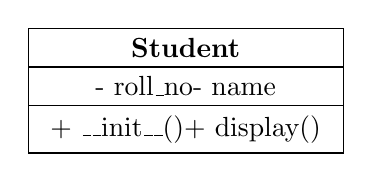
\begin{tikzpicture}
    \node[draw, rectangle split, rectangle split parts=3, minimum width=4cm] (student) {
        \textbf{Student}
        \nodepart{second}
        - roll\_no \newline
        - name
        \nodepart{third}
        + \_\_init\_\_() \newline
        + display()
    };
\end{tikzpicture}
\captionof{figure}{Class Diagram Example}
\end{center}

\begin{center}
\captionof{table}{OOP Concepts}
\begin{tabulary}{\linewidth}{|L|L|}
\hline
\textbf{Term} & \textbf{Description} \\ \hline
\textbf{Class} & Blueprint for creating objects with shared attributes and methods \\ \hline
\textbf{Attributes} & Variables that store data inside a class \\ \hline
\textbf{Object} & Instance of a class with specific attribute values \\ \hline
\textbf{Class Method} & Functions defined within a class that can access and modify class states \\ \hline
\end{tabulary}
\end{center}

\begin{lstlisting}[language=Python]
class Student:
    # Class attribute
    school = "GTU"
    
    # Constructor
    def __init__(self, roll_no, name):
        # Instance attributes
        self.roll_no = roll_no
        self.name = name
    
    # Instance method
    def display(self):
        print(f"Roll No: {self.roll_no}, Name: {self.name}")
    
    # Class method
    @classmethod
    def change_school(cls, new_school):
        cls.school = new_school

# Creating object
student1 = Student(101, "Raj")
student1.display()  # Output: Roll No: 101, Name: Raj
\end{lstlisting}
\end{solutionbox}

\begin{mnemonicbox}
\mnemonic{Class Creates, Attributes Store, Objects Use, Methods Operate}
\end{mnemonicbox}

\questionmarks{1(c) OR}{7}{Define Data Encapsulation \& Polymorphism. Develop a Python code to explain Polymorphism.}

\begin{solutionbox}
\begin{center}
\captionof{table}{Definitions}
\begin{tabulary}{\linewidth}{|L|L|}
\hline
\textbf{Concept} & \textbf{Definition} \\ \hline
\textbf{Data Encapsulation} & Bundling data and methods into a single unit (class) and restricting direct access to some components \\ \hline
\textbf{Polymorphism} & Ability of different classes to provide their own implementation of methods with the same name \\ \hline
\end{tabulary}
\end{center}

\begin{center}
\begin{tikzpicture}[
    level 1/.style={sibling distance=4cm},
    level 2/.style={sibling distance=2.5cm}
]
    \node[gtu block] {Polymorphism}
        child {node[gtu state] {Method Overriding}}
        child {node[gtu state] {Method Overloading}}
        child {node[gtu state] {Duck Typing}};
\end{tikzpicture}
\captionof{figure}{Types of Polymorphism}
\end{center}

\begin{lstlisting}[language=Python]
# Polymorphism example
class Animal:
    def speak(self):
        pass

class Dog(Animal):
    def speak(self):
        return "Woof!"

class Cat(Animal):
    def speak(self):
        return "Meow!"

class Duck(Animal):
    def speak(self):
        return "Quack!"

# Function demonstrating polymorphism
def animal_sound(animal):
    return animal.speak()

# Creating objects
dog = Dog()
cat = Cat()
duck = Duck()

# Same function works for different animal objects
print(animal_sound(dog))   # Output: Woof!
print(animal_sound(cat))   # Output: Meow!
print(animal_sound(duck))  # Output: Quack!
\end{lstlisting}
\end{solutionbox}

\begin{mnemonicbox}
\mnemonic{Encapsulate to Protect, Polymorphism for Flexibility}
\end{mnemonicbox}

\questionmarks{2(a)}{3}{Differentiate between Stack and Queue.}

\begin{solutionbox}
\begin{center}
\captionof{table}{Stack vs Queue}
\begin{tabulary}{\linewidth}{|L|L|L|}
\hline
\textbf{Feature} & \textbf{Stack} & \textbf{Queue} \\ \hline
\textbf{Principle} & LIFO (Last In First Out) & FIFO (First In First Out) \\ \hline
\textbf{Operations} & Push, Pop & Enqueue, Dequeue \\ \hline
\textbf{Access} & Elements can only be added/removed from one end (top) & Elements are added at rear end and removed from front end \\ \hline
\end{tabulary}
\end{center}

\begin{center}
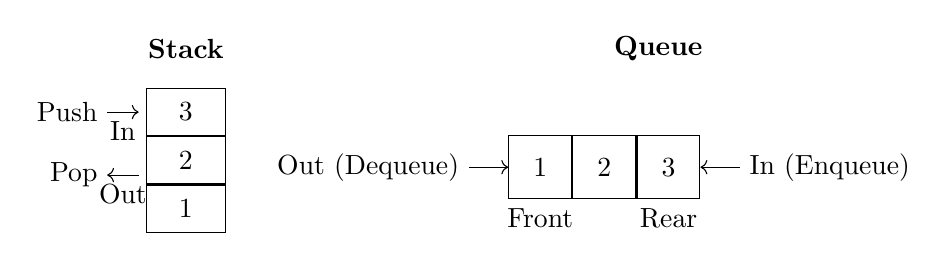
\begin{tikzpicture}[
    node distance=2cm,
    stacknode/.style={rectangle, draw, minimum width=1cm, minimum height=0.6cm},
    queuenode/.style={rectangle, draw, minimum size=0.8cm}
]
    % Stack
    \node at (-3, 2) {\textbf{Stack}};
    \node[stacknode] (s3) at (-3, 1.2) {3};
    \node[stacknode, below=0cm of s3] (s2) {2};
    \node[stacknode, below=0cm of s2] (s1) {1};
    \draw[->] (-4, 1.2) -- (-3.6, 1.2) node[left, pos=0] {Push} node[midway, below] {In};
    \draw[->] (-3.6, 0.4) -- (-4, 0.4) node[left, pos=1] {Pop} node[midway, below] {Out};

    % Queue
    \node at (3, 2) {\textbf{Queue}};
    \node[queuenode] (q1) at (1.5, 0.5) {1};
    \node[queuenode, right=0cm of q1] (q2) {2};
    \node[queuenode, right=0cm of q2] (q3) {3};
    \node[below] at (q1.south) {Front};
    \node[below] at (q3.south) {Rear};
    \draw[<-] (q1.west) -- ++(-0.5, 0) node[left] {Out (Dequeue)};
    \draw[<-] (q3.east) -- ++(0.5, 0) node[right] {In (Enqueue)};
\end{tikzpicture}
\captionof{figure}{Stack vs Queue Visual}
\end{center}
\end{solutionbox}

\begin{mnemonicbox}
\mnemonic{Stack Piles Up, Queue Lines Up}
\end{mnemonicbox}

\questionmarks{2(b)}{4}{Write an algorithm for PUSH and POP operation of stack in python.}

\begin{solutionbox}
\textbf{PUSH Algorithm:}
\begin{lstlisting}
Start
  1. Check if stack is full
  2. If not full, increment top by 1
  3. Add element at position 'top'
End
\end{lstlisting}

\textbf{POP Algorithm:}
\begin{lstlisting}
Start
  1. Check if stack is empty
  2. If not empty, retrieve element at 'top'
  3. Decrement top by 1
  4. Return retrieved element
End
\end{lstlisting}

\begin{lstlisting}[language=Python]
class Stack:
    def __init__(self, size):
        self.stack = []
        self.size = size
        self.top = -1
    
    def push(self, element):
        if self.top >= self.size - 1:
            return "Stack Overflow"
        else:
            self.top += 1
            self.stack.append(element)
            return "Pushed " + str(element)
    
    def pop(self):
        if self.top < 0:
            return "Stack Underflow"
        else:
            element = self.stack.pop()
            self.top -= 1
            return element
\end{lstlisting}
\end{solutionbox}

\begin{mnemonicbox}
\mnemonic{Push to Top, Pop from Top}
\end{mnemonicbox}

\questionmarks{2(c)}{7}{Convert following equation from infix to postfix using Stack. \newline
\textbf{A * (B + C) - D / (E + F)}}

\begin{solutionbox}
\begin{center}
\begin{tabulary}{\linewidth}{|L|L|}
\hline
\textbf{Infix} & $A * (B + C) - D / (E + F)$ \\ \hline
\textbf{Postfix} & $A B C + * D E F + / -$ \\ \hline
\end{tabulary}
\end{center}

\begin{center}
\captionof{table}{Infix to Postfix Conversion Trace}
\begin{tabulary}{\linewidth}{|C|C|L|L|}
\hline
\textbf{Step} & \textbf{Symbol} & \textbf{Stack} & \textbf{Output} \\ \hline
1 & A & & A \\ \hline
2 & * & * & A \\ \hline
3 & ( & * ( & A \\ \hline
4 & B & * ( & A B \\ \hline
5 & + & * ( + & A B \\ \hline
6 & C & * ( + & A B C \\ \hline
7 & ) & * & A B C + \\ \hline
8 & - & - & A B C + * \\ \hline
9 & D & - & A B C + * D \\ \hline
10 & / & - / & A B C + * D \\ \hline
11 & ( & - / ( & A B C + * D \\ \hline
12 & E & - / ( & A B C + * D E \\ \hline
13 & + & - / ( + & A B C + * D E \\ \hline
14 & F & - / ( + & A B C + * D E F \\ \hline
15 & ) & - / & A B C + * D E F + \\ \hline
16 & end & & A B C + * D E F + / - \\ \hline
\end{tabulary}
\end{center}

\textbf{Answer:} \code{A B C + * D E F + / -}
\end{solutionbox}

\begin{mnemonicbox}
\mnemonic{Operators Stack, Operands Print}
\end{mnemonicbox}

\questionmarks{2(a) OR}{3}{Differentiate between simple Queue and circular Queue.}

\begin{solutionbox}
\begin{center}
\captionof{table}{Simple vs Circular Queue}
\begin{tabulary}{\linewidth}{|L|L|L|}
\hline
\textbf{Feature} & \textbf{Simple Queue} & \textbf{Circular Queue} \\ \hline
\textbf{Structure} & Linear data structure & Linear data structure with connected ends \\ \hline
\textbf{Memory} & Inefficient memory usage due to unused space after dequeue & Efficient memory usage by reusing empty spaces \\ \hline
\textbf{Implementation} & Front always at index 0, rear increases & Front and rear move in circular fashion using modulo \\ \hline
\end{tabulary}
\end{center}

\begin{center}
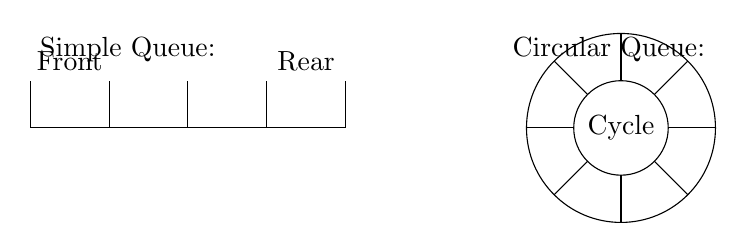
\begin{tikzpicture}
    % Simple Queue
    \node[anchor=west] at (-4, 1) {Simple Queue:};
    \draw (-4, 0) grid (0, 0.6);
    \node[above] at (-3.5, 0.6) {Front};
    \node[above] at (-0.5, 0.6) {Rear};

    % Circular Queue
    \node[anchor=west] at (2, 1) {Circular Queue:};
    \draw (3.5,0) circle [radius=1.2];
    \draw (3.5,0) circle [radius=0.6];
    \foreach \angle in {0, 45, ..., 315}
        \draw (3.5,0) ++(\angle:0.6) -- ++(\angle:0.6);
    \node at (3.5, 0) {Cycle};
\end{tikzpicture}
\captionof{figure}{Simple vs Circular Queue Structure}
\end{center}
\end{solutionbox}

\begin{mnemonicbox}
\mnemonic{Simple Wastes, Circular Reuses}
\end{mnemonicbox}

\questionmarks{2(b) OR}{4}{Explain concept of recursive function with suitable example.}

\begin{solutionbox}
\begin{center}
\captionof{table}{Recursive Function Concepts}
\begin{tabulary}{\linewidth}{|L|L|}
\hline
\textbf{Key Aspects} & \textbf{Description} \\ \hline
\textbf{Definition} & A function that calls itself to solve a smaller instance of the same problem \\ \hline
\textbf{Base Case} & The condition where the function stops calling itself \\ \hline
\textbf{Recursive Case} & The condition where the function calls itself with a simpler version of the problem \\ \hline
\end{tabulary}
\end{center}

\begin{center}
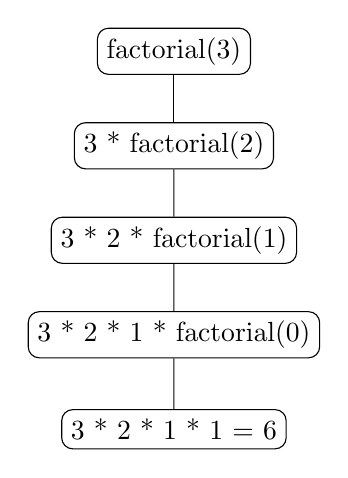
\begin{tikzpicture}[
    level distance=1.2cm,
    level 1/.style={sibling distance=4cm},
    every node/.style={rectangle, draw, rounded corners}
]
    \node {factorial(3)}
        child {node {3 * factorial(2)}
            child {node {3 * 2 * factorial(1)}
                child {node {3 * 2 * 1 * factorial(0)}
                    child {node {3 * 2 * 1 * 1 = 6}}
                }
            }
        };
\end{tikzpicture}
\captionof{figure}{Recursive Calls trace for factorial(3)}
\end{center}

\begin{lstlisting}[language=Python]
def factorial(n):
    # Base case
    if n == 0:
        return 1
    # Recursive case
    else:
        return n * factorial(n-1)

# Example
result = factorial(5)  # 5! = 120
\end{lstlisting}
\end{solutionbox}

\begin{mnemonicbox}
\mnemonic{Base Breaks, Recursion Returns}
\end{mnemonicbox}

\questionmarks{2(c) OR}{7}{Develop a python code to implement Enqueue and Dequeue operation in Queue.}

\begin{solutionbox}
\begin{center}
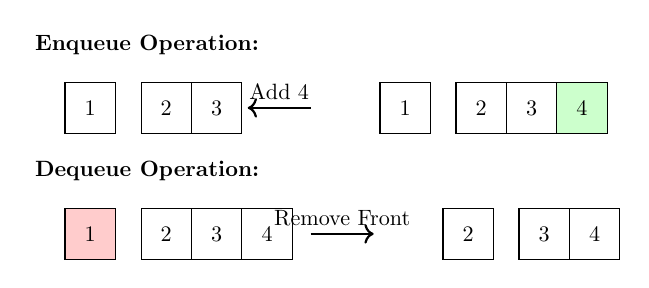
\begin{tikzpicture}[
    cell/.style={rectangle, draw, minimum size=0.8cm},
    scale=0.8, transform shape
]
    % Enqueue
    \node[anchor=west] at (-6, 2) {\textbf{Enqueue Operation:}};
    \node[cell] at (-5, 1) {1};
    \node[cell, right=0cm] at (-4.2, 1) {2};
    \node[cell, right=0cm] at (-3.4, 1) {3};
    \draw[->, thick] (-1.5, 1) -- (-2.5, 1) node[midway, above] {Add 4};
    \node[cell] at (0, 1) {1};
    \node[cell, right=0cm] at (0.8, 1) {2};
    \node[cell, right=0cm] at (1.6, 1) {3};
    \node[cell, right=0cm, fill=green!20] at (2.4, 1) {4};

    % Dequeue
    \node[anchor=west] at (-6, 0) {\textbf{Dequeue Operation:}};
    \node[cell, fill=red!20] at (-5, -1) {1};
    \node[cell, right=0cm] at (-4.2, -1) {2};
    \node[cell, right=0cm] at (-3.4, -1) {3};
    \node[cell, right=0cm] at (-2.6, -1) {4};
    \draw[->, thick] (-1.5, -1) -- (-0.5, -1) node[midway, above] {Remove Front};
    \node[cell] at (1, -1) {2};
    \node[cell, right=0cm] at (1.8, -1) {3};
    \node[cell, right=0cm] at (2.6, -1) {4};
\end{tikzpicture}
\captionof{figure}{Enqueue and Dequeue Visualization}
\end{center}

\begin{lstlisting}[language=Python]
class Queue:
    def __init__(self, size):
        self.queue = []
        self.size = size
        self.front = 0
        self.rear = -1
        self.count = 0
    
    def enqueue(self, item):
        if self.count >= self.size:
            return "Queue is full"
        else:
            self.rear += 1
            self.queue.append(item)
            self.count += 1
            return "Enqueued " + str(item)
    
    def dequeue(self):
        if self.count <= 0:
            return "Queue is empty"
        else:
            item = self.queue.pop(0)
            self.count -= 1
            return item
    
    def display(self):
        return self.queue

# Test
q = Queue(5)
q.enqueue(10)
q.enqueue(20)
q.enqueue(30)
print(q.display())  # [10, 20, 30]
print(q.dequeue())  # 10
print(q.display())  # [20, 30]
\end{lstlisting}
\end{solutionbox}

\begin{mnemonicbox}
\mnemonic{Enqueue at End, Dequeue from Start}
\end{mnemonicbox}

\questionmarks{3(a)}{3}{Give Difference between Singly linked list and Circular linked list.}

\begin{solutionbox}
\begin{center}
\captionof{table}{Singly vs Circular Linked List}
\begin{tabulary}{\linewidth}{|L|L|L|}
\hline
\textbf{Feature} & \textbf{Singly Linked List} & \textbf{Circular Linked List} \\ \hline
\textbf{Last Node} & Points to NULL & Points back to the first node \\ \hline
\textbf{Traversal} & Has a definite end & Can be traversed continuously \\ \hline
\textbf{Memory} & Each node needs one pointer & Each node needs one pointer \\ \hline
\end{tabulary}
\end{center}

\begin{center}
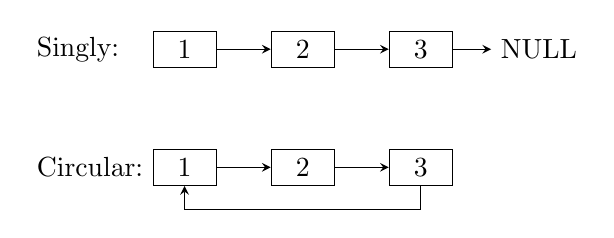
\begin{tikzpicture}[
    listnode/.style={rectangle, draw, minimum width=0.8cm},
    ptr/.style={->, >=stealth}
]
    % Singly
    \node[anchor=west] at (-2, 1) {Singly:};
    \node[listnode] (s1) at (0, 1) {1};
    \node[listnode] (s2) at (1.5, 1) {2};
    \node[listnode] (s3) at (3, 1) {3};
    \node (null) at (4.5, 1) {NULL};
    \draw[ptr] (s1) -- (s2);
    \draw[ptr] (s2) -- (s3);
    \draw[ptr] (s3) -- (null);

    % Circular
    \node[anchor=west] at (-2, -0.5) {Circular:};
    \node[listnode] (c1) at (0, -0.5) {1};
    \node[listnode] (c2) at (1.5, -0.5) {2};
    \node[listnode] (c3) at (3, -0.5) {3};
    \draw[ptr] (c1) -- (c2);
    \draw[ptr] (c2) -- (c3);
    \draw[ptr] (c3.south) -- ++(0,-0.3) -| (c1.south);
\end{tikzpicture}
\captionof{figure}{Singly vs Circular Structure}
\end{center}
\end{solutionbox}

\begin{mnemonicbox}
\mnemonic{Singly Stops, Circular Cycles}
\end{mnemonicbox}

\questionmarks{3(b)}{4}{Explain concept of Doubly linked list.}

\begin{solutionbox}
\begin{center}
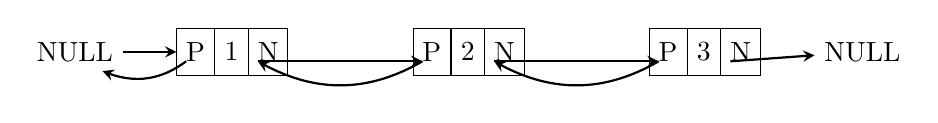
\begin{tikzpicture}[
    dnode/.style={rectangle split, rectangle split parts=3, draw, rectangle split horizontal, minimum height=0.6cm},
    ptr/.style={->, >=stealth, thick}
]
    \node[dnode] (n1) at (0,0) {\nodepart{one}P \nodepart{two}1 \nodepart{three}N};
    \node[dnode] (n2) at (3,0) {\nodepart{one}P \nodepart{two}2 \nodepart{three}N};
    \node[dnode] (n3) at (6,0) {\nodepart{one}P \nodepart{two}3 \nodepart{three}N};
    
    \node (start) at (-2, 0) {NULL};
    \node (end) at (8, 0) {NULL};

    \draw[ptr] (start) -- (n1.west);
    \draw[ptr] (n1.three) -- (n2.one);
    \draw[ptr] (n2.one) to[bend left] (n1.three); % Back pointer concept visually
    \draw[ptr] (n2.three) -- (n3.one);
    \draw[ptr] (n3.one) to[bend left] (n2.three);
    \draw[ptr] (n3.three) -- (end);

    % Correcting visualization for standard Doubly LL arrows
    \draw[ptr] (n1.one) to[bend left] (start);
\end{tikzpicture}
\captionof{figure}{Doubly Linked List Structure}
\end{center}

\begin{center}
\captionof{table}{Doubly Linked List Features}
\begin{tabulary}{\linewidth}{|L|L|}
\hline
\textbf{Feature} & \textbf{Description} \\ \hline
\textbf{Node Structure} & Each node contains data and two pointers (previous and next) \\ \hline
\textbf{Navigation} & Can traverse in both forward and backward directions \\ \hline
\textbf{Operations} & Insertion and deletion can be performed from both ends \\ \hline
\textbf{Memory Usage} & Requires more memory than singly linked list due to extra pointer \\ \hline
\end{tabulary}
\end{center}

\begin{lstlisting}[language=Python]
class Node:
    def __init__(self, data):
        self.data = data
        self.prev = None
        self.next = None
\end{lstlisting}
\end{solutionbox}

\begin{mnemonicbox}
\mnemonic{Double Pointers, Double Directions}
\end{mnemonicbox}

\questionmarks{3(c)}{7}{Write an algorithm for following operation on singly linked list: \newline
\textbf{1. To insert a node at the beginning of the list.} \newline
\textbf{2. To insert the node at the end of the list.}}

\begin{solutionbox}
\textbf{1. Insert at Beginning:}

\begin{center}
\begin{tikzpicture}[node distance=1.5cm, auto]
    \node[gtu block] (start) {Start};
    \node[gtu block, right=of start] (create) {Create new node};
    \node[gtu block, right=of create] (data) {Set data};
    \node[gtu block, below=of data] (next) {Set next to head};
    \node[gtu block, left=of next] (head) {Set head = new node};
    \node[gtu state, left=of head] (end) {End};

    \path[gtu arrow] (start) -- (create);
    \path[gtu arrow] (create) -- (data);
    \path[gtu arrow] (data) -- (next);
    \path[gtu arrow] (next) -- (head);
    \path[gtu arrow] (head) -- (end);
\end{tikzpicture}
\end{center}

\textbf{2. Insert at End:}

\begin{center}
\begin{tikzpicture}[node distance=1.5cm, auto]
    \node[gtu block] (start) {Start};
    \node[gtu block, right=of start] (create) {Create node};
    \node[gtu block, right=of create] (data) {Set data};
    \node[gtu block, below=of data] (next) {Set next=NULL};
    \node[gtu decision, left=of next] (check) {head is NULL?};
    \node[gtu block, below=of check] (sethead) {head = new node};
    \node[gtu block, left=of check] (traverse) {Traverse to last};
    \node[gtu block, below=of traverse] (link) {last.next = new node};
    \node[gtu state, left=of traverse] (end) {End};

    \path[gtu arrow] (start) -- (create);
    \path[gtu arrow] (create) -- (data);
    \path[gtu arrow] (data) -- (next);
    \path[gtu arrow] (next) -- (check);
    \path[gtu arrow] (check) -- node[right] {Yes} (sethead);
    \path[gtu arrow] (check) -- node[above] {No} (traverse);
    \path[gtu arrow] (traverse) -- (link);
    \path[gtu arrow] (sethead) -| (end);
    \path[gtu arrow] (link) -| (end);
\end{tikzpicture}
\end{center}

\begin{lstlisting}[language=Python]
def insert_at_beginning(head, data):
    new_node = Node(data)
    new_node.next = head
    return new_node  # New head

def insert_at_end(head, data):
    new_node = Node(data)
    new_node.next = None
    
    # If linked list is empty
    if head is None:
        return new_node
    
    # Traverse to the last node
    temp = head
    while temp.next:
        temp = temp.next
    
    # Link the last node to new node
    temp.next = new_node
    return head
\end{lstlisting}
\end{solutionbox}

\begin{mnemonicbox}
\mnemonic{Begin: New Leads Old, End: Old Leads New}
\end{mnemonicbox}

\questionmarks{3(a) OR}{3}{List different operations performed on singly linked list.}

\begin{solutionbox}
\begin{center}
\captionof{table}{Operations on Singly Linked List}
\begin{tabulary}{\linewidth}{|L|}
\hline
\textbf{Operations} \\ \hline
1. Insertion (at beginning, middle, end) \\ \hline
2. Deletion (from beginning, middle, end) \\ \hline
3. Traversal (visiting each node) \\ \hline
4. Searching (finding a specific node) \\ \hline
5. Updating (modifying node data) \\ \hline
\end{tabulary}
\end{center}

\begin{center}
\begin{tikzpicture}[
    level 1/.style={sibling distance=3.5cm},
    level 2/.style={sibling distance=2cm}
]
    \node[gtu block] {Linked List Operations}
        child {node[gtu state] {Insertion}}
        child {node[gtu state] {Deletion}}
        child {node[gtu state] {Traversal}}
        child {node[gtu state] {Searching}}
        child {node[gtu state] {Updating}};
\end{tikzpicture}
\captionof{figure}{LL Operations}
\end{center}
\end{solutionbox}

\begin{mnemonicbox}
\mnemonic{Insert Delete Traverse Search Update}
\end{mnemonicbox}

\questionmarks{3(b) OR}{4}{Explain concept of Circular linked list.}

\begin{solutionbox}
\begin{center}
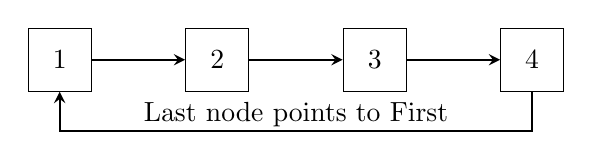
\begin{tikzpicture}[
    listnode/.style={rectangle, draw, minimum size=0.8cm},
    ptr/.style={->, >=stealth, thick}
]
    \node[listnode] (n1) at (0,0) {1};
    \node[listnode] (n2) at (2,0) {2};
    \node[listnode] (n3) at (4,0) {3};
    \node[listnode] (n4) at (6,0) {4};

    \draw[ptr] (n1) -- (n2);
    \draw[ptr] (n2) -- (n3);
    \draw[ptr] (n3) -- (n4);
    
    \draw[ptr] (n4.south) -- ++(0,-0.5) -| (n1.south);
    \node at (3, -0.7) {Last node points to First};
\end{tikzpicture}
\captionof{figure}{Circular Linked List Visualization}
\end{center}

\begin{center}
\captionof{table}{Circular LL Features}
\begin{tabulary}{\linewidth}{|L|L|}
\hline
\textbf{Feature} & \textbf{Description} \\ \hline
\textbf{Structure} & Last node points to the first node instead of NULL \\ \hline
\textbf{Advantage} & Allows continuous traversal through all nodes \\ \hline
\textbf{Applications} & Round robin scheduling, circular buffer implementation \\ \hline
\textbf{Operations} & Insertion and deletion similar to singly linked list with special handling for the last node \\ \hline
\end{tabulary}
\end{center}

\begin{lstlisting}[language=Python]
class Node:
    def __init__(self, data):
        self.data = data
        self.next = None

# Creating a circular linked list with 3 nodes
head = Node(1)
node2 = Node(2)
node3 = Node(3)

head.next = node2
node2.next = node3
node3.next = head  # Makes it circular
\end{lstlisting}
\end{solutionbox}

\begin{mnemonicbox}
\mnemonic{Last Links to First}
\end{mnemonicbox}

\questionmarks{3(c) OR}{7}{List application of linked list. Write an algorithm to count the number of nodes in singly linked list.}

\begin{solutionbox}
\begin{center}
\captionof{table}{Applications}
\begin{tabulary}{\linewidth}{|L|}
\hline
\textbf{Applications of Linked List} \\ \hline
1. Implementation of stacks and queues \\ \hline
2. Dynamic memory allocation \\ \hline
3. Undo functionality in applications \\ \hline
4. Hash tables (chaining) \\ \hline
5. Adjacency lists for graphs \\ \hline
\end{tabulary}
\end{center}

\textbf{Algorithm to Count Nodes:}
\begin{center}
\begin{tikzpicture}[node distance=1.5cm, auto]
    \node[gtu block] (start) {Start};
    \node[gtu block, right=of start] (init) {count = 0};
    \node[gtu block, right=of init] (temp) {temp = head};
    \node[gtu decision, below=of temp] (check) {temp != NULL?};
    \node[gtu block, left=of check] (inc) {count++};
    \node[gtu block, below=of inc] (next) {temp = temp.next};
    \node[gtu state, right=of check] (end) {Return count};

    \path[gtu arrow] (start) -- (init);
    \path[gtu arrow] (init) -- (temp);
    \path[gtu arrow] (temp) -- (check);
    \path[gtu arrow] (check) -- node[above] {Yes} (inc);
    \path[gtu arrow] (inc) -- (next);
    \path[gtu arrow] (next) -- (check.south);
    \path[gtu arrow] (check) -- node[above] {No} (end);
\end{tikzpicture}
\end{center}

\begin{lstlisting}[language=Python]
def count_nodes(head):
    count = 0
    temp = head
    
    while temp:
        count += 1
        temp = temp.next
    
    return count

# Example usage
# Assuming head points to the first node of a linked list
total_nodes = count_nodes(head)
print(f"Total nodes: {total_nodes}")
\end{lstlisting}
\end{solutionbox}

\begin{mnemonicbox}
\mnemonic{Count While Moving}
\end{mnemonicbox}

\questionmarks{4(a)}{3}{Compare Linear search with Binary search.}

\begin{solutionbox}
\begin{center}
\captionof{table}{Linear vs Binary Search}
\begin{tabulary}{\linewidth}{|L|L|L|}
\hline
\textbf{Feature} & \textbf{Linear Search} & \textbf{Binary Search} \\ \hline
\textbf{Data Arrangement} & Works on both sorted and unsorted data & Works only on sorted data \\ \hline
\textbf{Time Complexity} & O(n) & O(log n) \\ \hline
\textbf{Implementation} & Simpler & More complex \\ \hline
\textbf{Best For} & Small datasets or unsorted data & Large sorted datasets \\ \hline
\end{tabulary}
\end{center}

\begin{center}
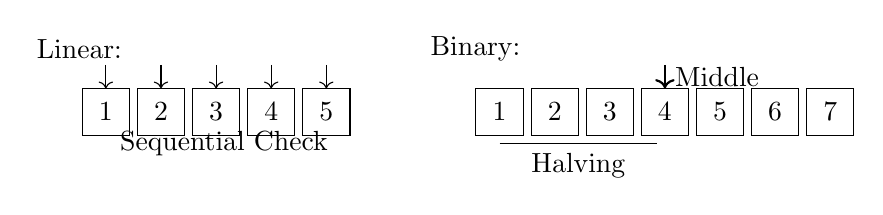
\begin{tikzpicture}
    % Linear
    \node[anchor=west] at (-4, 2) {Linear:};
    \foreach \x/\val in {0/1, 1/2, 2/3, 3/4, 4/5} {
        \node[draw, rectangle, minimum size=0.6cm] at (-3+\x*0.7, 1.2) {\val};
        \draw[->] (-3+\x*0.7, 1.8) -- (-3+\x*0.7, 1.5);
    }
    \node at (-1.5, 0.8) {Sequential Check};

    % Binary
    \node[anchor=west] at (1, 2) {Binary:};
    \foreach \x/\val in {0/1, 1/2, 2/3, 3/4, 4/5, 5/6, 6/7} {
        \node[draw, rectangle, minimum size=0.6cm] at (2+\x*0.7, 1.2) {\val};
    }
    \draw[->, thick] (2+3*0.7, 1.8) -- (2+3*0.7, 1.5) node[midway, right] {Middle};
    \draw (2, 0.8) -- (4, 0.8) node[midway, below] {Halving};
\end{tikzpicture}
\captionof{figure}{Search Comparison}
\end{center}
\end{solutionbox}

\begin{mnemonicbox}
\mnemonic{Linear Looks at All, Binary Breaks in Half}
\end{mnemonicbox}

\questionmarks{4(b)}{4}{Write an algorithm for selection sort method.}

\begin{solutionbox}
\textbf{Visualization:}
\begin{center}
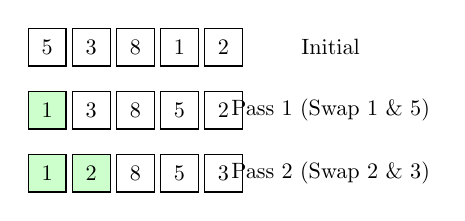
\begin{tikzpicture}[
    arrnode/.style={draw, rectangle, minimum size=0.6cm},
    scale=0.8, transform shape
]
    \node[arrnode] at (0, 3) {5}; \node[arrnode] at (0.7, 3) {3}; \node[arrnode] at (1.4, 3) {8}; \node[arrnode] at (2.1, 3) {1}; \node[arrnode] at (2.8, 3) {2};
    \node at (4.5, 3) {Initial};

    \node[arrnode, fill=green!20] at (0, 2) {1}; \node[arrnode] at (0.7, 2) {3}; \node[arrnode] at (1.4, 2) {8}; \node[arrnode] at (2.1, 2) {5}; \node[arrnode] at (2.8, 2) {2};
    \node at (4.5, 2) {Pass 1 (Swap 1 \& 5)};

    \node[arrnode, fill=green!20] at (0, 1) {1}; \node[arrnode, fill=green!20] at (0.7, 1) {2}; \node[arrnode] at (1.4, 1) {8}; \node[arrnode] at (2.1, 1) {5}; \node[arrnode] at (2.8, 1) {3};
    \node at (4.5, 1) {Pass 2 (Swap 2 \& 3)};
\end{tikzpicture}
\end{center}

\textbf{Algorithm:}
\begin{center}
\begin{tikzpicture}[node distance=1.5cm]
    \node[gtu block] (start) {Start};
    \node[gtu block, right=of start] (loop) {For i = 0 to n-1};
    \node[gtu block, right=of loop] (find) {Find min in unsorted};
    \node[gtu block, below=of find] (swap) {Swap min with arr[i]};
    \node[gtu state, left=of swap] (end) {End};

    \path[gtu arrow] (start) -- (loop);
    \path[gtu arrow] (loop) -- (find);
    \path[gtu arrow] (find) -- (swap);
    \path[gtu arrow] (swap) -- (end);
\end{tikzpicture}
\end{center}

\begin{lstlisting}[language=Python]
def selection_sort(arr):
    n = len(arr)
    
    for i in range(n):
        min_idx = i
        
        # Find the minimum element in unsorted array
        for j in range(i+1, n):
            if arr[j] < arr[min_idx]:
                min_idx = j
        
        # Swap the found minimum element with the first element
        arr[i], arr[min_idx] = arr[min_idx], arr[i]
\end{lstlisting}
\end{solutionbox}

\begin{mnemonicbox}
\mnemonic{Find Minimum, Swap Position}
\end{mnemonicbox}

\questionmarks{4(c)}{7}{Develop a python code to sort following list in ascending order using Bubble sort method. \newline
\textbf{list1=[5,4,3,2,1,0]}}

\begin{solutionbox}
\begin{center}
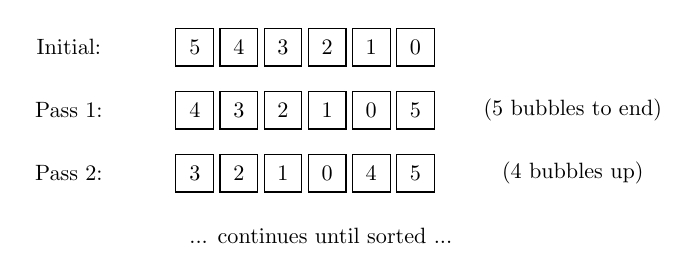
\begin{tikzpicture}[
    arrnode/.style={draw, rectangle, minimum size=0.6cm},
    scale=0.8, transform shape
]
    \node at (-2, 2.5) {Initial:};
    \foreach \x/\val in {0/5, 1/4, 2/3, 3/2, 4/1, 5/0} \node[arrnode] at (\x*0.7, 2.5) {\val};

    \node at (-2, 1.5) {Pass 1:};
    \foreach \x/\val in {0/4, 1/3, 2/2, 3/1, 4/0, 5/5} \node[arrnode] at (\x*0.7, 1.5) {\val};
    \node at (6, 1.5) {(5 bubbles to end)};

    \node at (-2, 0.5) {Pass 2:};
    \foreach \x/\val in {0/3, 1/2, 2/1, 3/0, 4/4, 5/5} \node[arrnode] at (\x*0.7, 0.5) {\val};
    \node at (6, 0.5) {(4 bubbles up)};
    
    \node at (2, -0.5) {... continues until sorted ...};
\end{tikzpicture}
\captionof{figure}{Bubble Sort Trace}
\end{center}

\begin{lstlisting}[language=Python]
def bubble_sort(arr):
    n = len(arr)
    
    # Traverse through all array elements
    for i in range(n):
        # Last i elements are already in place
        for j in range(0, n-i-1):
            # Swap if current element is greater than next element
            if arr[j] > arr[j+1]:
                arr[j], arr[j+1] = arr[j+1], arr[j]
    
    return arr

# Input list
list1 = [5, 4, 3, 2, 1, 0]

# Sorting the list
sorted_list = bubble_sort(list1)

# Displaying the result
print("Sorted list:", sorted_list)
# Output: Sorted list: [0, 1, 2, 3, 4, 5]
\end{lstlisting}
\end{solutionbox}

\begin{mnemonicbox}
\mnemonic{Bubble Biggest Upward}
\end{mnemonicbox}

\questionmarks{4(a) OR}{3}{Define sorting. List different sorting methods.}

\begin{solutionbox}
\begin{center}
\captionof{table}{Sorting Definition}
\begin{tabulary}{\linewidth}{|L|L|}
\hline
\textbf{Definition} & \textbf{Sorting Methods} \\ \hline
Sorting is the process of arranging data in a specified order (ascending or descending) & 1. Bubble Sort \newline 2. Selection Sort \newline 3. Insertion Sort \newline 4. Merge Sort \newline 5. Quick Sort \newline 6. Heap Sort \newline 7. Radix Sort \\ \hline
\end{tabulary}
\end{center}

\begin{center}
\begin{tikzpicture}[
    level 1/.style={sibling distance=4cm},
    level 2/.style={sibling distance=1.5cm}
]
    \node[gtu block] {Sorting Algorithms}
        child {node[gtu block] {Comparison-based}
            child {node[gtu state] {Bubble}}
            child {node[gtu state] {Selection}}
            child {node[gtu state] {Insertion}}
            child {node[gtu state] {Merge}}
            child {node[gtu state] {Quick}}
        }
        child {node[gtu block] {Non-comparison}
            child {node[gtu state] {Counting}}
            child {node[gtu state] {Radix}}
            child {node[gtu state] {Bucket}}
        };
\end{tikzpicture}
\captionof{figure}{Hierarchy of Sorting Algorithms}
\end{center}
\end{solutionbox}

\begin{mnemonicbox}
\mnemonic{Better Sort Improves Many Query Results}
\end{mnemonicbox}

\questionmarks{4(b) OR}{4}{Write an algorithm for Insertion sort method.}

\begin{solutionbox}
\textbf{Visualization:}
\begin{center}
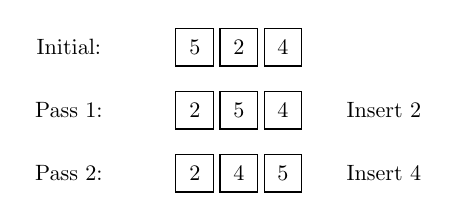
\begin{tikzpicture}[
    arrnode/.style={draw, rectangle, minimum size=0.6cm},
    scale=0.8, transform shape
]
    \node at (0, 3) {Initial:}; \foreach \x/\val in {0/5, 1/2, 2/4} \node[arrnode] at (2+\x*0.7, 3) {\val};
    \node at (0, 2) {Pass 1:}; \foreach \x/\val in {0/2, 1/5, 2/4} \node[arrnode] at (2+\x*0.7, 2) {\val}; \node at (5, 2) {Insert 2};
    \node at (0, 1) {Pass 2:}; \foreach \x/\val in {0/2, 1/4, 2/5} \node[arrnode] at (2+\x*0.7, 1) {\val}; \node at (5, 1) {Insert 4};
\end{tikzpicture}
\end{center}

\textbf{Algorithm Flow:}
\begin{center}
\begin{tikzpicture}[node distance=1.2cm]
    \node[gtu block] (start) {Start};
    \node[gtu block, right=of start] (loop) {For i=1 to n-1};
    \node[gtu block, right=of loop] (key) {key = arr[i]};
    \node[gtu decision, below=of key] (check) {arr[j] > key?};
    \node[gtu block, left=of check] (move) {Move right};
    \node[gtu block, below=of check] (place) {Place key};
    \node[gtu state, left=of place] (end) {End};

    \path[gtu arrow] (start) -- (loop);
    \path[gtu arrow] (loop) -- (key);
    \path[gtu arrow] (key) -- (check);
    \path[gtu arrow] (check) -- node[above] {Yes} (move);
    \path[gtu arrow] (move) |- (check);
    \path[gtu arrow] (check) -- node[right] {No} (place);
    \path[gtu arrow] (place) -- (end);
\end{tikzpicture}
\end{center}

\begin{lstlisting}[language=Python]
def insertion_sort(arr):
    for i in range(1, len(arr)):
        key = arr[i]
        j = i - 1
        
        # Move elements that are greater than key
        # to one position ahead of their current position
        while j >= 0 and arr[j] > key:
            arr[j + 1] = arr[j]
            j -= 1
        
        arr[j + 1] = key
\end{lstlisting}
\end{solutionbox}

\begin{mnemonicbox}
\mnemonic{Take Card, Insert In Order}
\end{mnemonicbox}

\questionmarks{4(c) OR}{7}{Develop a python code to sort following list in ascending order using selection sort method. \newline
\textbf{list1=[6,3,25,8,-1,55,0]}}

\begin{solutionbox}
\begin{center}
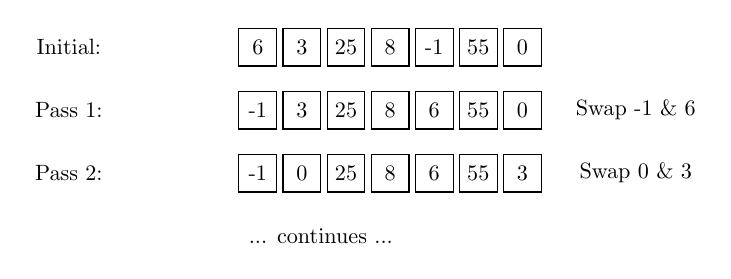
\begin{tikzpicture}[
    arrnode/.style={draw, rectangle, minimum size=0.6cm},
    scale=0.8, transform shape
]
    \node at (-1, 3.5) {Initial:};
    \foreach \x/\val in {0/6, 1/3, 2/25, 3/8, 4/-1, 5/55, 6/0} \node[arrnode] at (2+\x*0.7, 3.5) {\val};

    \node at (-1, 2.5) {Pass 1:};
    \foreach \x/\val in {0/-1, 1/3, 2/25, 3/8, 4/6, 5/55, 6/0} \node[arrnode] at (2+\x*0.7, 2.5) {\val};
    \node at (8, 2.5) {Swap -1 \& 6};

    \node at (-1, 1.5) {Pass 2:};
    \foreach \x/\val in {0/-1, 1/0, 2/25, 3/8, 4/6, 5/55, 6/3} \node[arrnode] at (2+\x*0.7, 1.5) {\val};
    \node at (8, 1.5) {Swap 0 \& 3};

    \node at (3, 0.5) {... continues ...};
\end{tikzpicture}
\captionof{figure}{Selection Sort Trace}
\end{center}

\begin{lstlisting}[language=Python]
def selection_sort(arr):
    n = len(arr)
    
    for i in range(n):
        # Find the minimum element in remaining unsorted array
        min_idx = i
        for j in range(i+1, n):
            if arr[j] < arr[min_idx]:
                min_idx = j
                
        # Swap the found minimum element with the first element
        arr[i], arr[min_idx] = arr[min_idx], arr[i]
    
    return arr

# Input list
list1 = [6, 3, 25, 8, -1, 55, 0]

# Sorting the list
sorted_list = selection_sort(list1)

# Displaying the result
print("Sorted list:", sorted_list)
# Output: Sorted list: [-1, 0, 3, 6, 8, 25, 55]
\end{lstlisting}
\end{solutionbox}

\begin{mnemonicbox}
\mnemonic{Select Smallest, Shift to Start}
\end{mnemonicbox}

\questionmarks{5(a)}{3}{Define following terms regarding Tree data structure: \newline
\textbf{1. Forest} \newline
\textbf{2. Root node} \newline
\textbf{3. Leaf node}}

\begin{solutionbox}
\begin{center}
\captionof{table}{Tree Terminology}
\begin{tabulary}{\linewidth}{|L|L|}
\hline
\textbf{Term} & \textbf{Definition} \\ \hline
\textbf{Forest} & Collection of disjoint trees (multiple trees without connections between them) \\ \hline
\textbf{Root Node} & Topmost node of a tree with no parent, from which all other nodes are descended \\ \hline
\textbf{Leaf Node} & Node with no children (terminal node at the bottom of the tree) \\ \hline
\end{tabulary}
\end{center}

\begin{center}
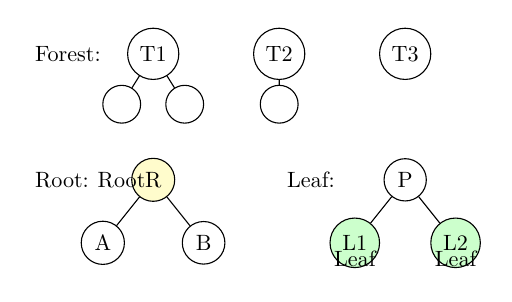
\begin{tikzpicture}[
    treenode/.style={circle, draw, minimum size=0.6cm},
    scale=0.8, transform shape
]
    % Forest
    \node[anchor=west] at (-2, 2) {Forest:};
    \node[treenode] (t1) at (0, 2) {T1}; \node[treenode] (t1a) at (-0.5, 1.2) {}; \node[treenode] (t1b) at (0.5, 1.2) {}; \draw (t1)--(t1a); \draw (t1)--(t1b);
    \node[treenode] (t2) at (2, 2) {T2}; \node[treenode] (t2a) at (2, 1.2) {}; \draw (t2)--(t2a);
    \node[treenode] (t3) at (4, 2) {T3};

    % Root
    \node[anchor=west] at (-2, 0) {Root:};
    \node[treenode, fill=yellow!20] (r) at (0, 0) {R};
    \node[treenode] (c1) at (-0.8, -1) {A}; \node[treenode] (c2) at (0.8, -1) {B};
    \draw (r)--(c1); \draw (r)--(c2);
    \node[left] at (r) {Root};

    % Leaf
    \node[anchor=west] at (2, 0) {Leaf:};
    \node[treenode] (p) at (4, 0) {P};
    \node[treenode, fill=green!20] (l1) at (3.2, -1) {L1}; \node[treenode, fill=green!20] (l2) at (4.8, -1) {L2};
    \draw (p)--(l1); \draw (p)--(l2);
    \node[below] at (l1) {Leaf}; \node[below] at (l2) {Leaf};
\end{tikzpicture}
\captionof{figure}{Tree Terms Visualization}
\end{center}
\end{solutionbox}

\begin{mnemonicbox}
\mnemonic{Forest has Many Roots, Roots Lead All, Leaves End All}
\end{mnemonicbox}

\questionmarks{5(b)}{4}{Draw Binary search tree for 78, 58, 82, 15, 66, 80, 99 and write In-order traversal for the tree.}

\begin{solutionbox}
\begin{center}
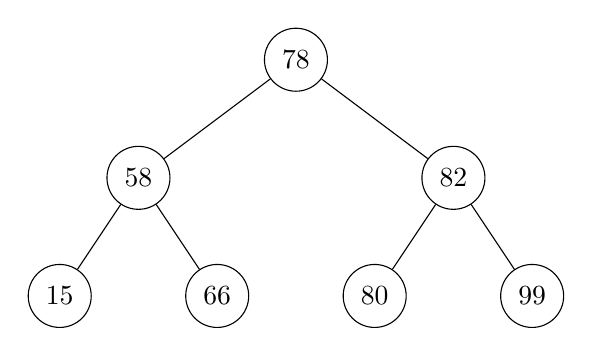
\begin{tikzpicture}[
    level distance=1.5cm,
    level 1/.style={sibling distance=4cm},
    level 2/.style={sibling distance=2cm},
    every node/.style={circle, draw, minimum size=0.8cm}
]
    \node {78}
        child {node {58}
            child {node {15}}
            child {node {66}}
        }
        child {node {82}
            child {node {80}}
            child {node {99}}
        };
\end{tikzpicture}
\captionof{figure}{Binary Search Tree for Given Data}
\end{center}

\textbf{In-order Traversal:}
\begin{center}
\begin{tabulary}{\linewidth}{|C|L|}
\hline
\textbf{Step} & \textbf{Visit Order} \\ \hline
1 & Visit left subtree of 78 \\ \hline
2 & Visit left subtree of 58 \\ \hline
3 & Visit 15 \\ \hline
4 & Visit 58 \\ \hline
5 & Visit 66 \\ \hline
6 & Visit 78 \\ \hline
7 & Visit left subtree of 82 \\ \hline
8 & Visit 80 \\ \hline
9 & Visit 82 \\ \hline
10 & Visit 99 \\ \hline
\end{tabulary}
\end{center}

\textbf{In-order Traversal Result: 15, 58, 66, 78, 80, 82, 99}
\end{solutionbox}

\begin{mnemonicbox}
\mnemonic{Left, Root, Right}
\end{mnemonicbox}

\questionmarks{5(c)}{7}{Write an algorithm for following operation: \newline
\textbf{1. Insertion of Node in Binary Tree} \newline
\textbf{2. Deletion of Node in Binary Tree}}

\begin{solutionbox}
\textbf{Insertion Algorithm:}
\begin{center}
\begin{tikzpicture}[node distance=1.5cm]
    \node[gtu block] (start) {Start};
    \node[gtu block, right=of start] (create) {Create Node};
    \node[gtu decision, right=of create] (check) {Root NULL?};
    \node[gtu block, below=of check] (setroot) {Set Root};
    \node[gtu block, right=of check] (find) {Find empty (Bfs)};
    \node[gtu block, below=of find] (insert) {Insert Node};
    \node[gtu state, below=of setroot] (end) {End};

    \path[gtu arrow] (start) -- (create);
    \path[gtu arrow] (create) -- (check);
    \path[gtu arrow] (check) -- node[right] {Yes} (setroot);
    \path[gtu arrow] (check) -- node[above] {No} (find);
    \path[gtu arrow] (find) -- (insert);
    \path[gtu arrow] (setroot) -- (end);
    \path[gtu arrow] (insert) |- (end);
\end{tikzpicture}
\end{center}

\textbf{Deletion Algorithm:}
\begin{center}
\begin{tikzpicture}[node distance=1.5cm]
    \node[gtu block] (start) {Start};
    \node[gtu decision, right=of start] (empty) {Tree empty?};
    \node[gtu state, below=of empty] (ret) {Return};
    \node[gtu block, right=of empty] (find) {Find node};
    \node[gtu block, right=of find] (deep) {Find deepest right};
    \node[gtu block, below=of deep] (repl) {Replace data};
    \node[gtu block, left=of repl] (del) {Delete deepest};
    \node[gtu state, left=of del] (end) {End};

    \path[gtu arrow] (start) -- (empty);
    \path[gtu arrow] (empty) -- node[right] {Yes} (ret);
    \path[gtu arrow] (empty) -- node[above] {No} (find);
    \path[gtu arrow] (find) -- (deep);
    \path[gtu arrow] (deep) -- (repl);
    \path[gtu arrow] (repl) -- (del);
    \path[gtu arrow] (del) -- (end);
\end{tikzpicture}
\end{center}

\begin{lstlisting}[language=Python]
class Node:
    def __init__(self, data):
        self.data = data
        self.left = None
        self.right = None

# Insertion in Binary Tree
def insert(root, data):
    if root is None:
        return Node(data)
    
    # Level order traversal to find vacant position
    queue = []
    queue.append(root)
    
    while queue:
        temp = queue.pop(0)
        
        if temp.left is None:
            temp.left = Node(data)
            break
        else:
            queue.append(temp.left)
            
        if temp.right is None:
            temp.right = Node(data)
            break
        else:
            queue.append(temp.right)
    
    return root

# Deletion in Binary Tree
def delete_node(root, key):
    if root is None:
        return None
    
    if root.left is None and root.right is None:
        if root.data == key:
            return None
        else:
            return root
    
    # Find the node to delete and deepest node
    key_node = None
    last = None
    parent = None
    queue = []
    queue.append(root)
    
    while queue:
        temp = queue.pop(0)
        if temp.data == key:
            key_node = temp
        if temp.left:
            parent = temp
            queue.append(temp.left)
            last = temp.left
        if temp.right:
            parent = temp
            queue.append(temp.right)
            last = temp.right
    
    if key_node:
        key_node.data = last.data
        if parent.right == last:
            parent.right = None
        else:
            parent.left = None
    
    return root
\end{lstlisting}
\end{solutionbox}

\begin{mnemonicbox}
\mnemonic{Insert at Empty, Delete by Swap and Remove}
\end{mnemonicbox}

\questionmarks{5(a) OR}{3}{Define following terms regarding Tree data structure: \newline
\textbf{1. In-degree} \newline
\textbf{2. Out-degree} \newline
\textbf{3. Depth}}

\begin{solutionbox}
\begin{center}
\captionof{table}{Definitions}
\begin{tabulary}{\linewidth}{|L|L|}
\hline
\textbf{Term} & \textbf{Definition} \\ \hline
\textbf{In-degree} & Number of edges coming into a node (always 1 for each node except root node in a tree) \\ \hline
\textbf{Out-degree} & Number of edges going out from a node (number of children) \\ \hline
\textbf{Depth} & Length of the path from root to the node (number of edges in path) \\ \hline
\end{tabulary}
\end{center}

\begin{center}
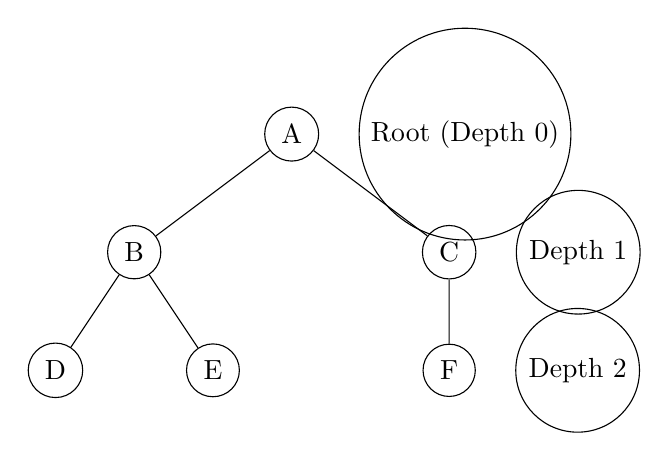
\begin{tikzpicture}[
    level distance=1.5cm,
    level 1/.style={sibling distance=4cm},
    level 2/.style={sibling distance=2cm},
    every node/.style={circle, draw}
]
    \node (a) {A}
        child {node (b) {B}
            child {node (d) {D}}
            child {node (e) {E}}
        }
        child {node (c) {C}
            child {node (f) {F}}
        };
    
    \node[right=0.5cm of a] {Root (Depth 0)};
    \node[right=0.5cm of c] {Depth 1};
    \node[right=0.5cm of f] {Depth 2};
\end{tikzpicture}
\captionof{figure}{Tree Depth and Degrees}
\end{center}

\begin{center}
\captionof{table}{Degree Analysis}
\begin{tabulary}{\linewidth}{|C|C|C|}
\hline
\textbf{Node} & \textbf{In-degree} & \textbf{Out-degree} \\ \hline
A & 0 & 2 \\ \hline
B & 1 & 2 \\ \hline
C & 1 & 1 \\ \hline
D & 1 & 0 \\ \hline
E & 1 & 0 \\ \hline
F & 1 & 0 \\ \hline
\end{tabulary}
\end{center}
\end{solutionbox}

\begin{mnemonicbox}
\mnemonic{In Counts Parents, Out Counts Children, Depth Counts Edges from Root}
\end{mnemonicbox}

\questionmarks{5(b) OR}{4}{Write Preorder and postorder traversal of following Binary tree. \newline
\textbf{100 -> (20 -> (10, 30), 200 -> (150, 300))}}

\begin{solutionbox}
\begin{center}
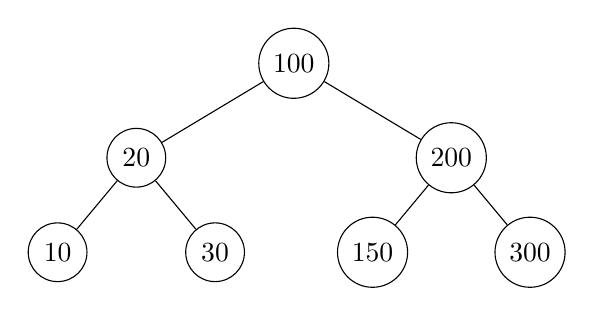
\begin{tikzpicture}[
    level distance=1.2cm,
    level 1/.style={sibling distance=4cm},
    level 2/.style={sibling distance=2cm},
    every node/.style={circle, draw}
]
    \node {100}
        child {node {20}
            child {node {10}}
            child {node {30}}
        }
        child {node {200}
            child {node {150}}
            child {node {300}}
        };
\end{tikzpicture}
\captionof{figure}{Given Binary Tree}
\end{center}

\begin{center}
\captionof{table}{Traversals}
\begin{tabulary}{\linewidth}{|L|L|L|}
\hline
\textbf{Traversal} & \textbf{Order} & \textbf{Result} \\ \hline
\textbf{Preorder} & Root, Left, Right & 100, 20, 10, 30, 200, 150, 300 \\ \hline
\textbf{Postorder} & Left, Right, Root & 10, 30, 20, 150, 300, 200, 100 \\ \hline
\end{tabulary}
\end{center}
\end{solutionbox}

\begin{mnemonicbox}
\mnemonic{Preorder: Root First, Postorder: Children First}
\end{mnemonicbox}

\questionmarks{5(c) OR}{7}{Develop a program to implement construction of Binary Search Tree.}

\begin{solutionbox}
\textbf{Construction Visualization:}
\begin{center}
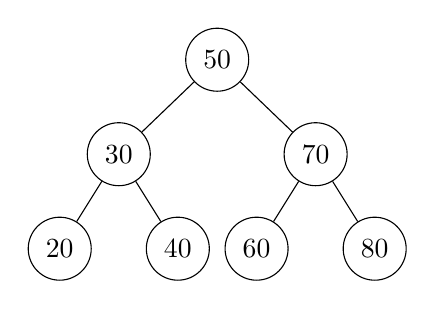
\begin{tikzpicture}[
    every node/.style={circle, draw, minimum size=0.8cm},
    level distance=1.2cm,
    level 1/.style={sibling distance=2.5cm},
    level 2/.style={sibling distance=1.5cm}
]
    \node {50}
        child {node {30}
            child {node {20}}
            child {node {40}}
        }
        child {node {70}
            child {node {60}}
            child {node {80}}
        };
\end{tikzpicture}
\captionof{figure}{BST Constructed from [50, 30, 20, 40, 70, 60, 80]}
\end{center}

\begin{lstlisting}[language=Python]
class Node:
    def __init__(self, key):
        self.key = key
        self.left = None
        self.right = None

def insert(root, key):
    # If the tree is empty, return a new node
    if root is None:
        return Node(key)
    
    # Otherwise, recur down the tree
    if key < root.key:
        root.left = insert(root.left, key)
    else:
        root.right = insert(root.right, key)
    
    # Return the unchanged node pointer
    return root

def inorder(root):
    if root:
        inorder(root.left)
        print(root.key, end=" ")
        inorder(root.right)

def preorder(root):
    if root:
        print(root.key, end=" ")
        preorder(root.left)
        preorder(root.right)

def postorder(root):
    if root:
        postorder(root.left)
        postorder(root.right)
        print(root.key, end=" ")

# Driver program to test the above functions
def main():
    # Create BST with these elements: 50, 30, 20, 40, 70, 60, 80
    root = None
    elements = [50, 30, 20, 40, 70, 60, 80]
    
    for element in elements:
        root = insert(root, element)
    
    # Print traversals
    print("Inorder traversal: ", end="")
    inorder(root)
    print("\nPreorder traversal: ", end="")
    preorder(root)
    print("\nPostorder traversal: ", end="")
    postorder(root)

# Run the program
main()
\end{lstlisting}

\textbf{Example Output:}
\begin{lstlisting}
Inorder traversal: 20 30 40 50 60 70 80
Preorder traversal: 50 30 20 40 70 60 80
Postorder traversal: 20 40 30 60 80 70 50
\end{lstlisting}
\end{solutionbox}

\begin{mnemonicbox}
\mnemonic{Insert Smaller Left, Larger Right}
\end{mnemonicbox}

\end{document}



